\newpage
\chapter{Results}
\label{experiment_results}
\lhead{\emph{Experimental Results}}
We first present a full replication and extension of the work by
\citet{radDeliberationSinglePeakednessCoherent2021}. Then we present the simulations based on our model of
meta-deliberation, as well as the results of the sensitivity analysis on both
models.


\section{Replication}\label{sec: replication}

We successfully replicate the results found by
\citet{radDeliberationSinglePeakednessCoherent2021}.  \Cref{fig:rep_cyclic}
shows for biases less than 0.73, all metrics result in acyclic preferences. We also
replicate the behavior of the KS metric, where biases in the range of
0.73-0.85, show that even initially acyclic profiles can become cyclic. This is
further illustrated in \Cref{fig:rep_count}, showing that within this range we
always observe 3 unique preferences for the KS metric, while DP and CS always
have 6 unique preferences, thereby representing all possible preferences.
Finally, the proximity to single-peakedness shows a slightly more positive note
for the KS metric, showing that while the DP and CS bottom out to the minimum
proximity to single-peakedness, KS stays relatively high. However, this should
be interpreted cautiously, as it likely reflects the smaller number of unique
preferences, and thus the number of voters that need to be removed is at most
1/3.

\begin{figure}[htbp]
	\centering
	\begin{minipage}{0.45\textwidth}
		\centering
		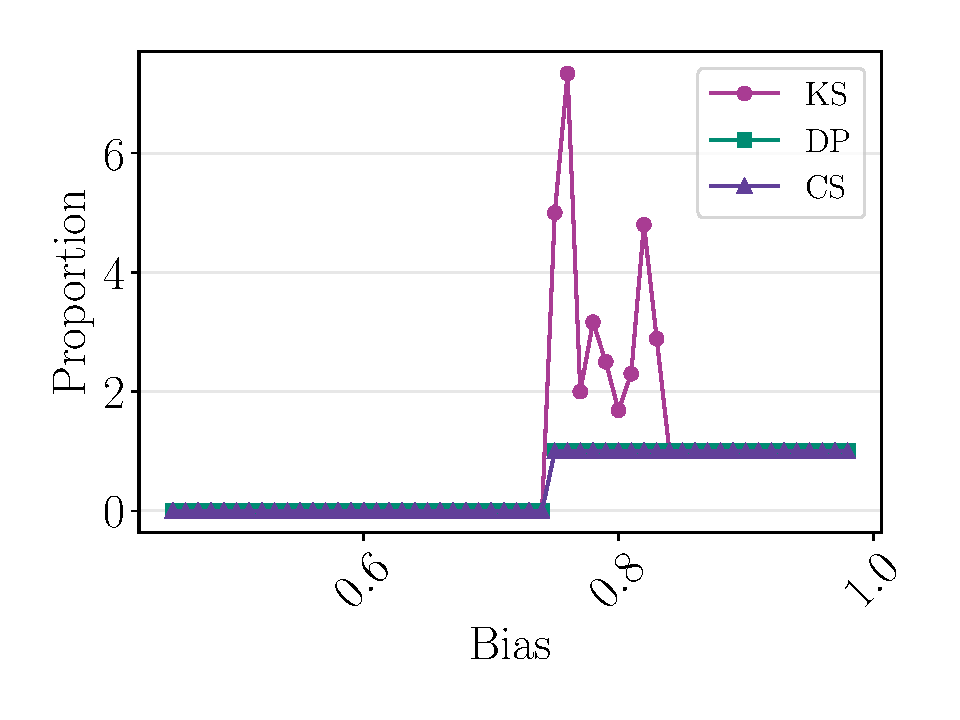
\includegraphics[width=\textwidth]{Figures/cyclic_proportion_Proportion.pdf}
		\caption{The proportion of cyclic profiles remaining, 0 indicating that no cyclic profiles were present after deliberation.}
		\label{fig:rep_cyclic}
	\end{minipage}\hfill
	\begin{minipage}{0.45\textwidth}
		\centering
		\vspace{-9pt}
		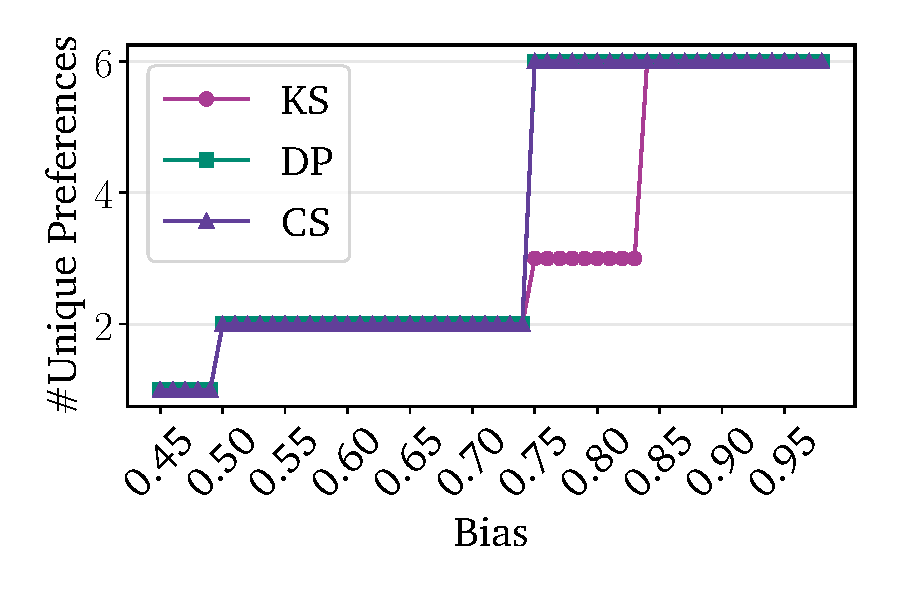
\includegraphics[width=\textwidth]{Figures/unique_Unique Preferences.pdf}
		\caption{Number of unique preferences at the final step of deliberation.}
		\label{fig:rep_count}
	\end{minipage}

	\vspace{1em}

	\begin{minipage}{0.45\textwidth}
		\centering
		\vspace{-9pt}
		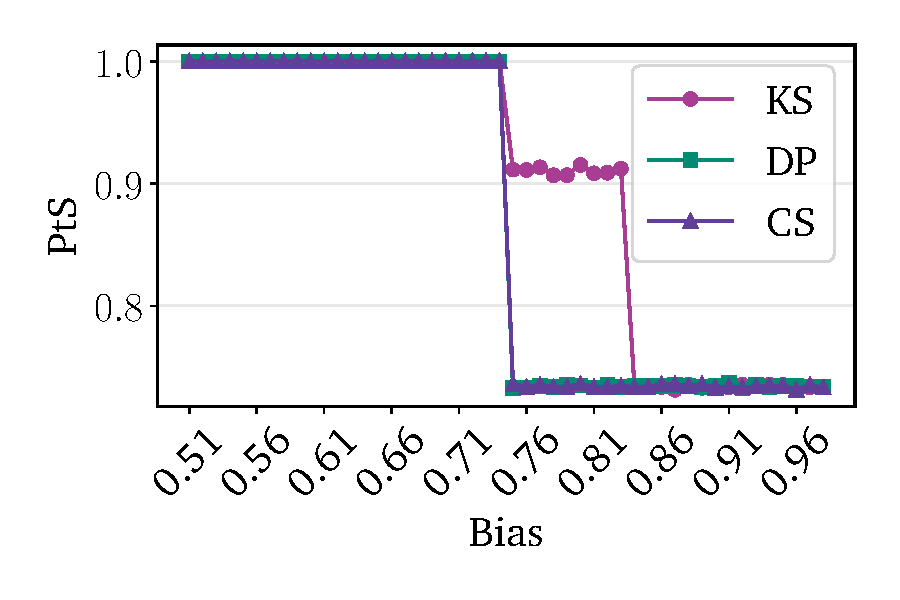
\includegraphics[width=\textwidth]{Figures/sp_proximity_PtS.pdf}
		\caption{Proximity to single-peakedness after deliberation. Proximity to single-peakedness as defined in \Cref{section:related_work}.}
		\label{fig:rep_single_peaked}
	\end{minipage}
\end{figure}

Through these results, we observe that while the original model does show
increase in the proximity to single-peakedness (PtS-V) and discourages cyclic
profiles, its outcomes are highly sensitive to both voter bias and the chosen
distance metric. In particular, the instability observed with the KS metric
across certain bias ranges raises concerns about the robustness and external
validity of the approach. Moreover, the model lacks a mechanism for
higher-order disagreement or reflection—there is no ``meta'' level at which
agents evaluate the structure of their preferences. This limitation motivates
the development of our own model, which explicitly incorporates
meta-deliberation and trust dynamics to better capture the complexities of
real-world opinion formation.

\newpage
\section{DeGroot Model}\label{degroot_results}

% Intro
The model is calibrated using the data from the \textsc{America in one Room}
experiment, which was used to construct the support vectors $\Support_i$ (each
voter's vector of policy opinions), where each element in $\Support_i$
corresponds to one response in the questionnaire. We follow the original paper,
focussing on the 26 most polarizing questions, which we then use to calculate
the policy-based ideology score (PBS) as the average these polarizing
questions. Low PBS corresponds to more liberal answers, and high PBS indicates
more conservative answers.

We remove all participants with missing responses to any pre- or
post-deliberation measurements, retaining only participants with complete pre-
and post-deliberation data. As a result, only 247 out of the original 523
opinions remain after this selection. This removes a large fraction of
participants. However, it limits the number of assumptions we have to make on
the opinions of participants.  Interpolation of the missing data would likely
artificially inflate the accuracy of the model, this might be further
exaggerated by the fact that we need to infer preferences over (artificial)
candidates.

The support vectors $\Support_i$ correspond to the participants' reported
opinions, based on measured by several policy questions rated from 0 to 10
(inclusive). Each voter's estimated support matrix $\EstSupport$ is generated
by adding normally distributed noise($\mu=0$, $\sigma=1.37$) to the candidates'
true opinions. Ensuring the model does not systematically favor candidates with
higher or lower average scores, as otherwise voters would on average be over
or underestimating candidates' support. The standard deviation is chosen to
match voter PBS distribution before deliberation. The opinions of the
candidates are generated as mentioned in \Cref{method: meta-agreement}, namely by copying the
opinion of a voter at random, or by sampling ten voters with replacement.


% Simulation parameters
To generate a deliberation group, we opt for two approaches. Either using the
original deliberation groups, selecting a group at random and using the
participants from that group. Given the restriction of voters with complete
data these groups will tend to be smaller than in the original study, where
these groups averaged 13 voters, in our subsection the average is 7. Or we
generate new groups by picking $n$ voters uniformly at random without
replacement.

To evaluate model performance, we predict each voter's post-deliberation PBS
and compare it to the observed data. Additionally, we group voters into ten bins
based on their initial PBS and compare the average predicted PBS within each
bin to the true bin average. This approach effectively models deliberation the
substantive level and thus does not yet incorporate the possibility of
\textit{meta-agreement}. However, it allows for the evaluation of the model
without assumptions on how to infer the final preferences of the voters, or
the opinions of candidates. After this assessment, we investigate the
convergence of the model, as well as its sensitivity to the choice of
parameters.

% Extension to meta agreement
Finally, we extend the model to incorporate meta-deliberation through deliberation
on the estimated support matrices. Assessing its effect on voters’ final preferences, using
the metrics introduced in \Cref{method: meta-agreement}.

\subsection{Policy-Based Ideology Scores}

We first proceed with analyzing the performance of the DeGroot model with
respect to substantive agreement. \Cref{fig:pbs} shows the PBS of both the
deliberation and control group, and the simulation results for both instances,
here the results are averaged over all tested configurations of the model. The
trust matrix for the control group is generated using the network of citations
in physics \cite{nr}, and is sampled down to the size of the number of voters
using the TIES sampling technique
\cite{ahmedNetworkSamplingStatic2013}\footnote{To address the issue of
	assigning voters to nodes in the final sampled graph (see
	\Cref{theory}), we used a Fast Approximate Quadratic Assignment Problem
	solver \cite{vogelsteinFastApproximateQuadratic2015}. However, this
	approach did not consistently outperform random initialization.}. As expected
the model has high mean absolute error (MAE) when predicting the post
deliberation PBS of the control group, as there was no significant change for
control group members in the original data. Within the deliberation group, a
voter's initial PBS remains a strong indicator of their final PBS. We observe
that the models predictions get more accurate after the first time step, with
prediction errors increasing over time. This is because the model causes voters
to converge too strongly, thereby eliminating most extreme opinions, contrary
to the real data. The implications of this depend on the nature of long term
deliberation. If, as suggested by \citet{elsterMarketForumThree2002},
deliberation is able to reach full consensus, the model might offer a plausible
approximation of this process. However, if full consensus is not typically
reached—as is precisely the motivation for incorporating meta-agreement into
the model—then the DeGroot model should be seen as overly simplistic in its
assumption that individuals converge toward a weighted average of the opinions
presented to them.

\begin{figure}[ht]
	\begin{center}
		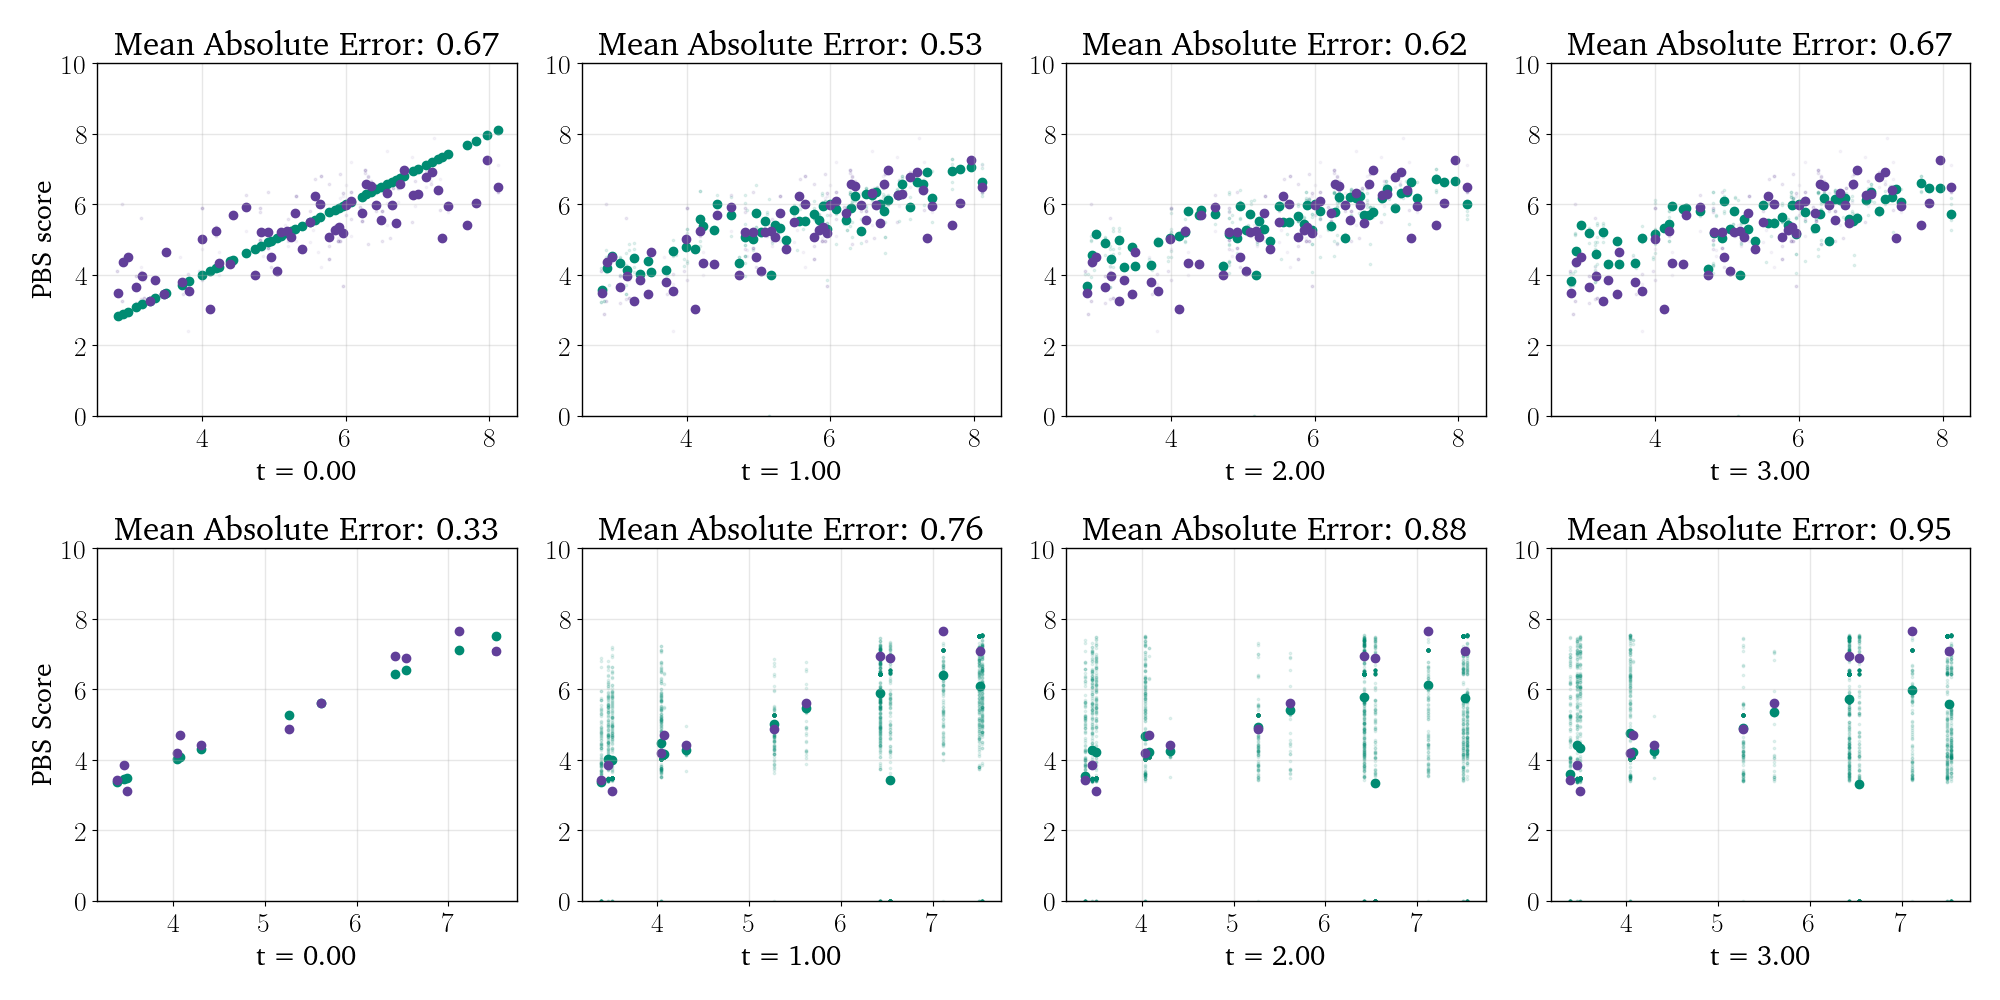
\includegraphics[width=0.95\textwidth]{Figures/pbs_scores.png}
	\end{center}
	\caption{ PBS, purple indicating the PBS after deliberation in the original data, green indicates the results of the simulation in that time step. Large dots indicate the binned data, smaller dots indicate individual voters.}\label{fig:pbs}
\end{figure}

\Cref{fig:delta_pbs} depicts the change in PBS within the deliberation
group. In the original data, most changes occur among participants
with high initial PBS, who tend to moderate their views. The model, by
contrast, predicts the most change among those with low PBS.

One possible explanation for this discrepancy is the correlation between PBS
and political knowledge. As shown by
\citet{fishkinCanDeliberationHave2024}, voters with more extreme PBS also tend
to be more knowledgeable. Our filtered dataset supports this, showing a weak
negative correlation of -0.05 ($p < 0.05$), \Cref{fig:knowledge_pbs}
in~\Cref{AppendixA} shows the distribution of political knowledge across
different PBS ranges. Since political knowledge in our sample is skewed toward
voters with high PBS, incorporating knowledge-based trust into the model
amplifies their influence, resulting in larger prediction errors.



\begin{figure}[ht]
	\begin{center}
		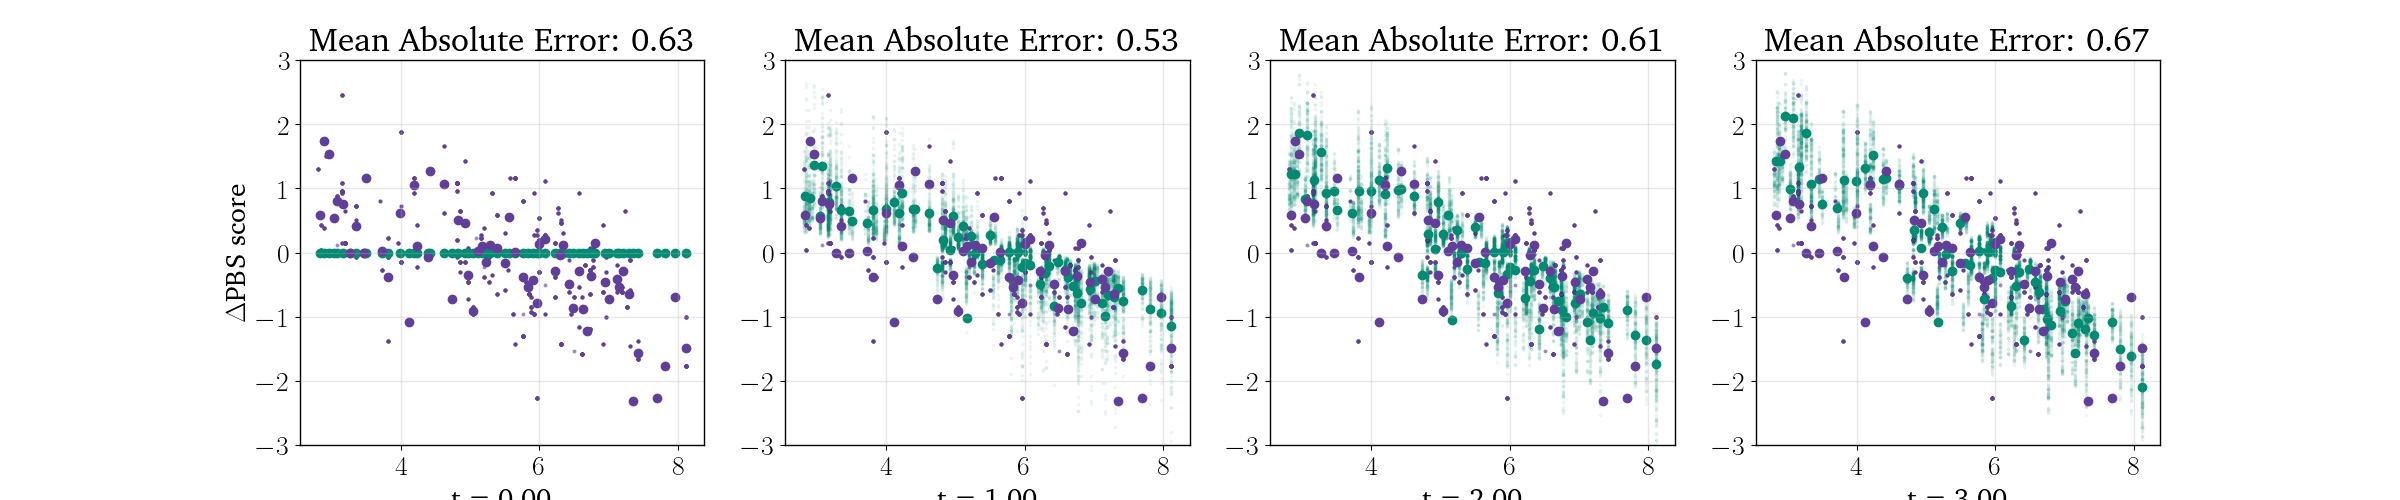
\includegraphics[width=\textwidth]{Figures/change_pbs_scores.png}
	\end{center}
	\caption{Change in  PBS, relative to the original, pre deliberation, measurement. The control is  omitted as there was no significant change.}\label{fig:delta_pbs}
\end{figure}


We note that these positive results appear only when the voters are grouped by
their original PBS during the initial 3-4 time steps, thereby giving the model
reasonable predictive power over a population of voters. \Cref{fig:binned_errors} shows the progression of errors over
time when the error is calculated on a per-individual basis (left), and binned
(right). We find the model does not predict the change per individual well,
with the original score at t=0 being a better predictor of an individual's final
PBS than the model's output during any subsequent time steps. Notably, using the ego-based trust, the model makes
smaller prediction errors. When we look at the predictions binned by initial
PBS, the model seems to be doing a lot better, again with ego-based trust
resulting in the lowest error. Interestingly after the first time step,
knowledge-based trust results in the lowest prediction error, after this step
ego-based trust outperforms all other kinds of trust.

Furthermore, \Cref{fig:binned_errors} shows that the model predicts individual PBS changes it has higher MAE when
knowledge is included in the trust calculation as opposed to Ego, and is equal
to similarity. This suggests that political knowledge, at least as measured in
this dataset, is a poor predictor of persuasiveness. As he knowledge questions
assess factual knowledge of the U.S. government, such as knowing which party
holds a Senate majority, knowledge may not correlate well with persuasiveness on
specific policy issues such as immigration or the economy.


\begin{figure}[ht]
	\begin{center}
		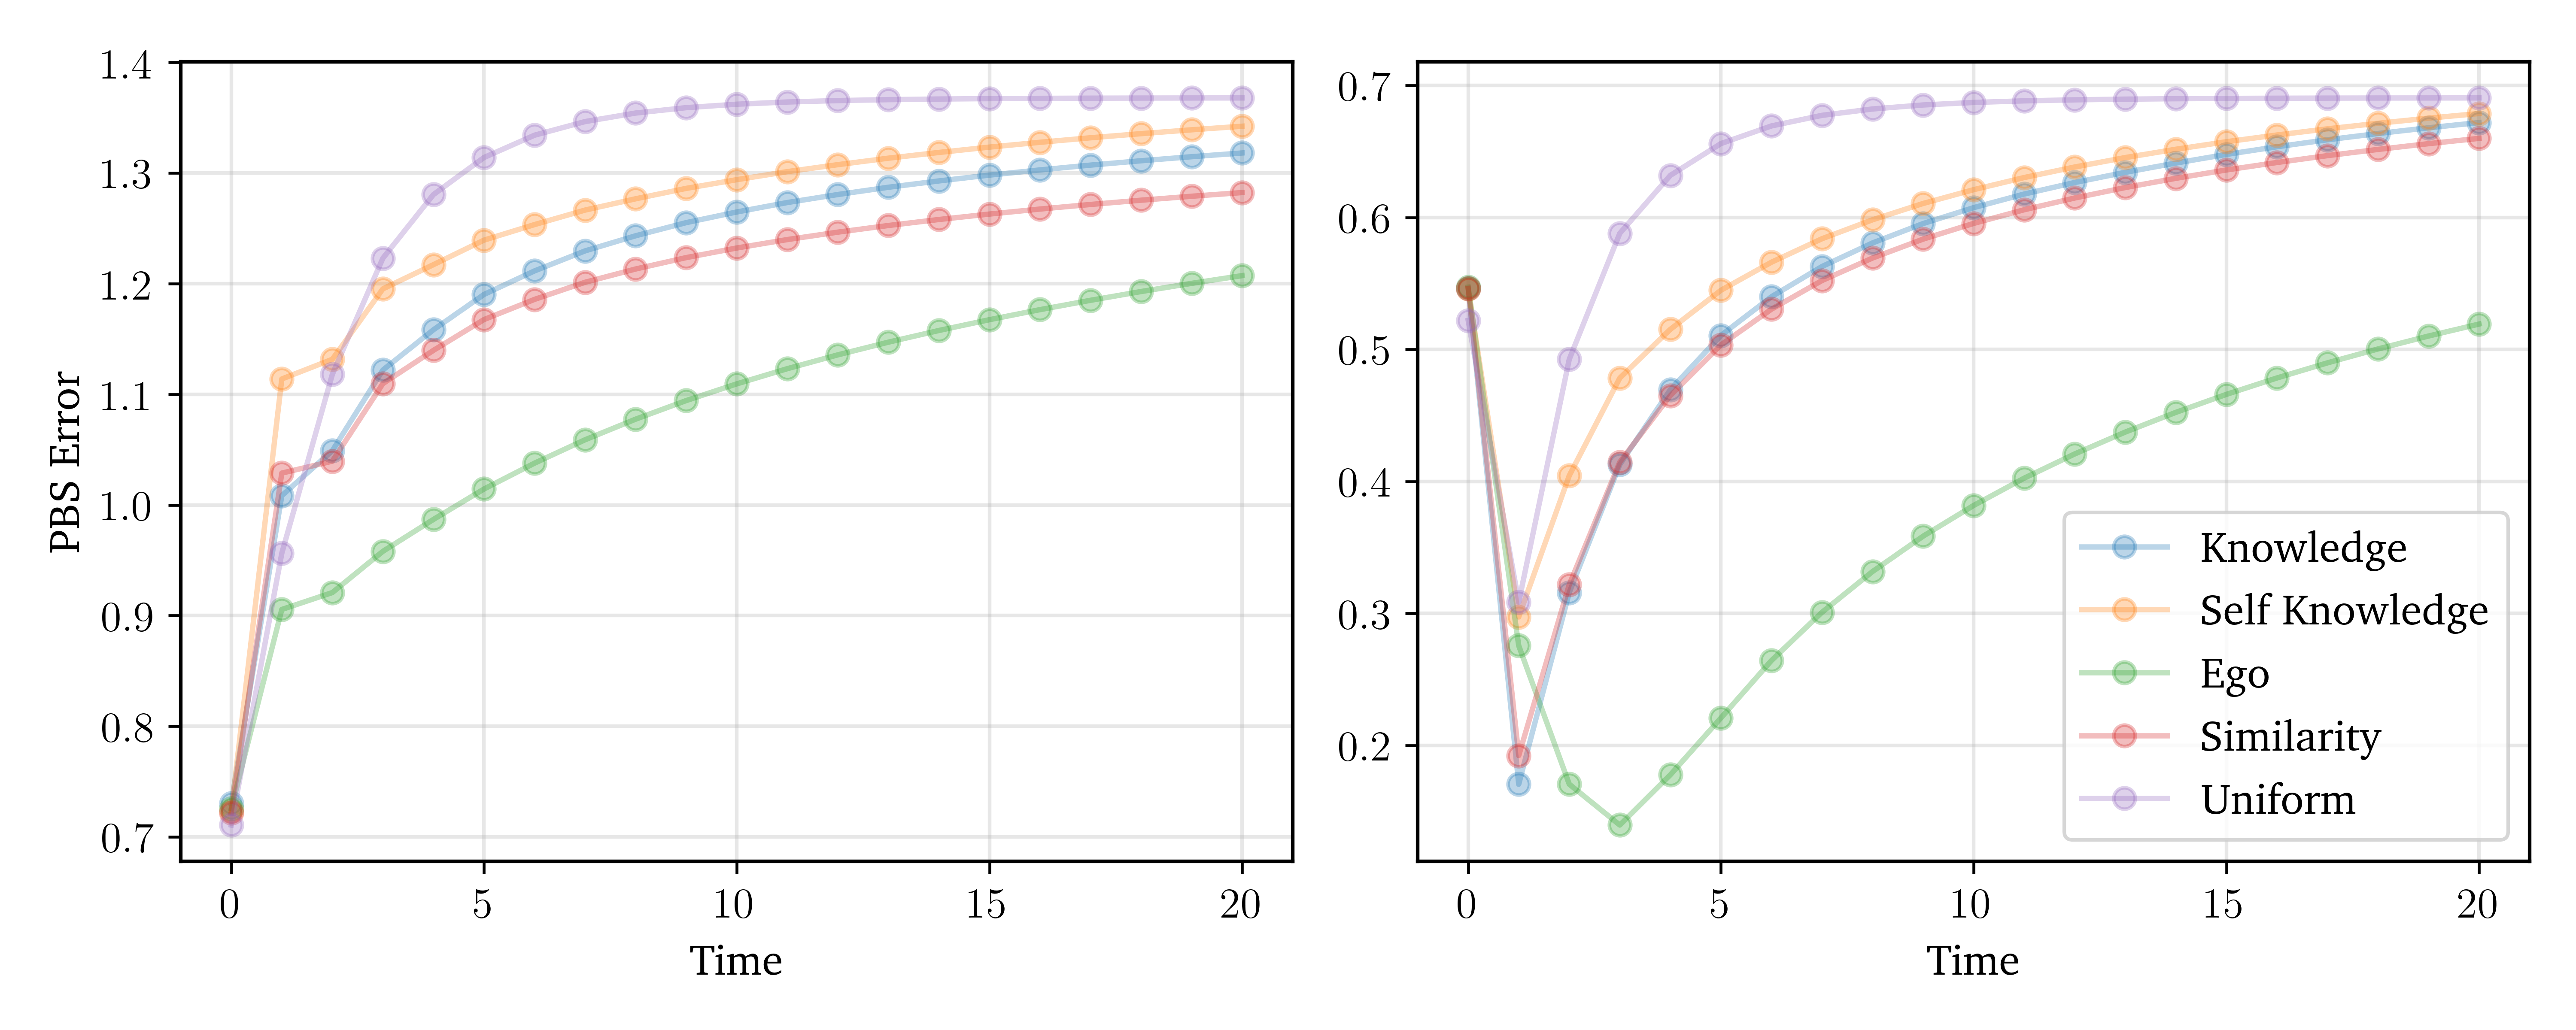
\includegraphics[width=0.95\textwidth]{Figures/errors_binned.png}
	\end{center}
	\caption{(Left) Mean absolute prediction error over time for different
		trust mechanisms, with 95\% confidence intervals at each time step.
		(Right) Mean absolute error binned by voters' initial PBS score. Binning
		reveals how predictive performance varies across the ideological
		spectrum.}\label{fig:binned_errors}
\end{figure}


Further, looking into the change in PBS, \Cref{fig:per_topic} divides the
change in PBS up into the change on each topic measured. The model predicts the
change in PBS for healthcare very well across different trust generation methods, as well as
changing the PBS into the right direction for the economy and immigration,
still the model predicts roughly half as much change in PBS for immigration for
any of the trust generation methods. For the environment and
foreign policy, the model predicted an increase in PBS on average,
while in reality people decreased their PBS. Comparing different trust
generation methods, we see that ego and similarity are quite similar on most
topics, but specifically on the economy ego seems to be very accurate, while
similarity does not seem to lead to significant change.

\begin{figure}[ht]
	\begin{center}
		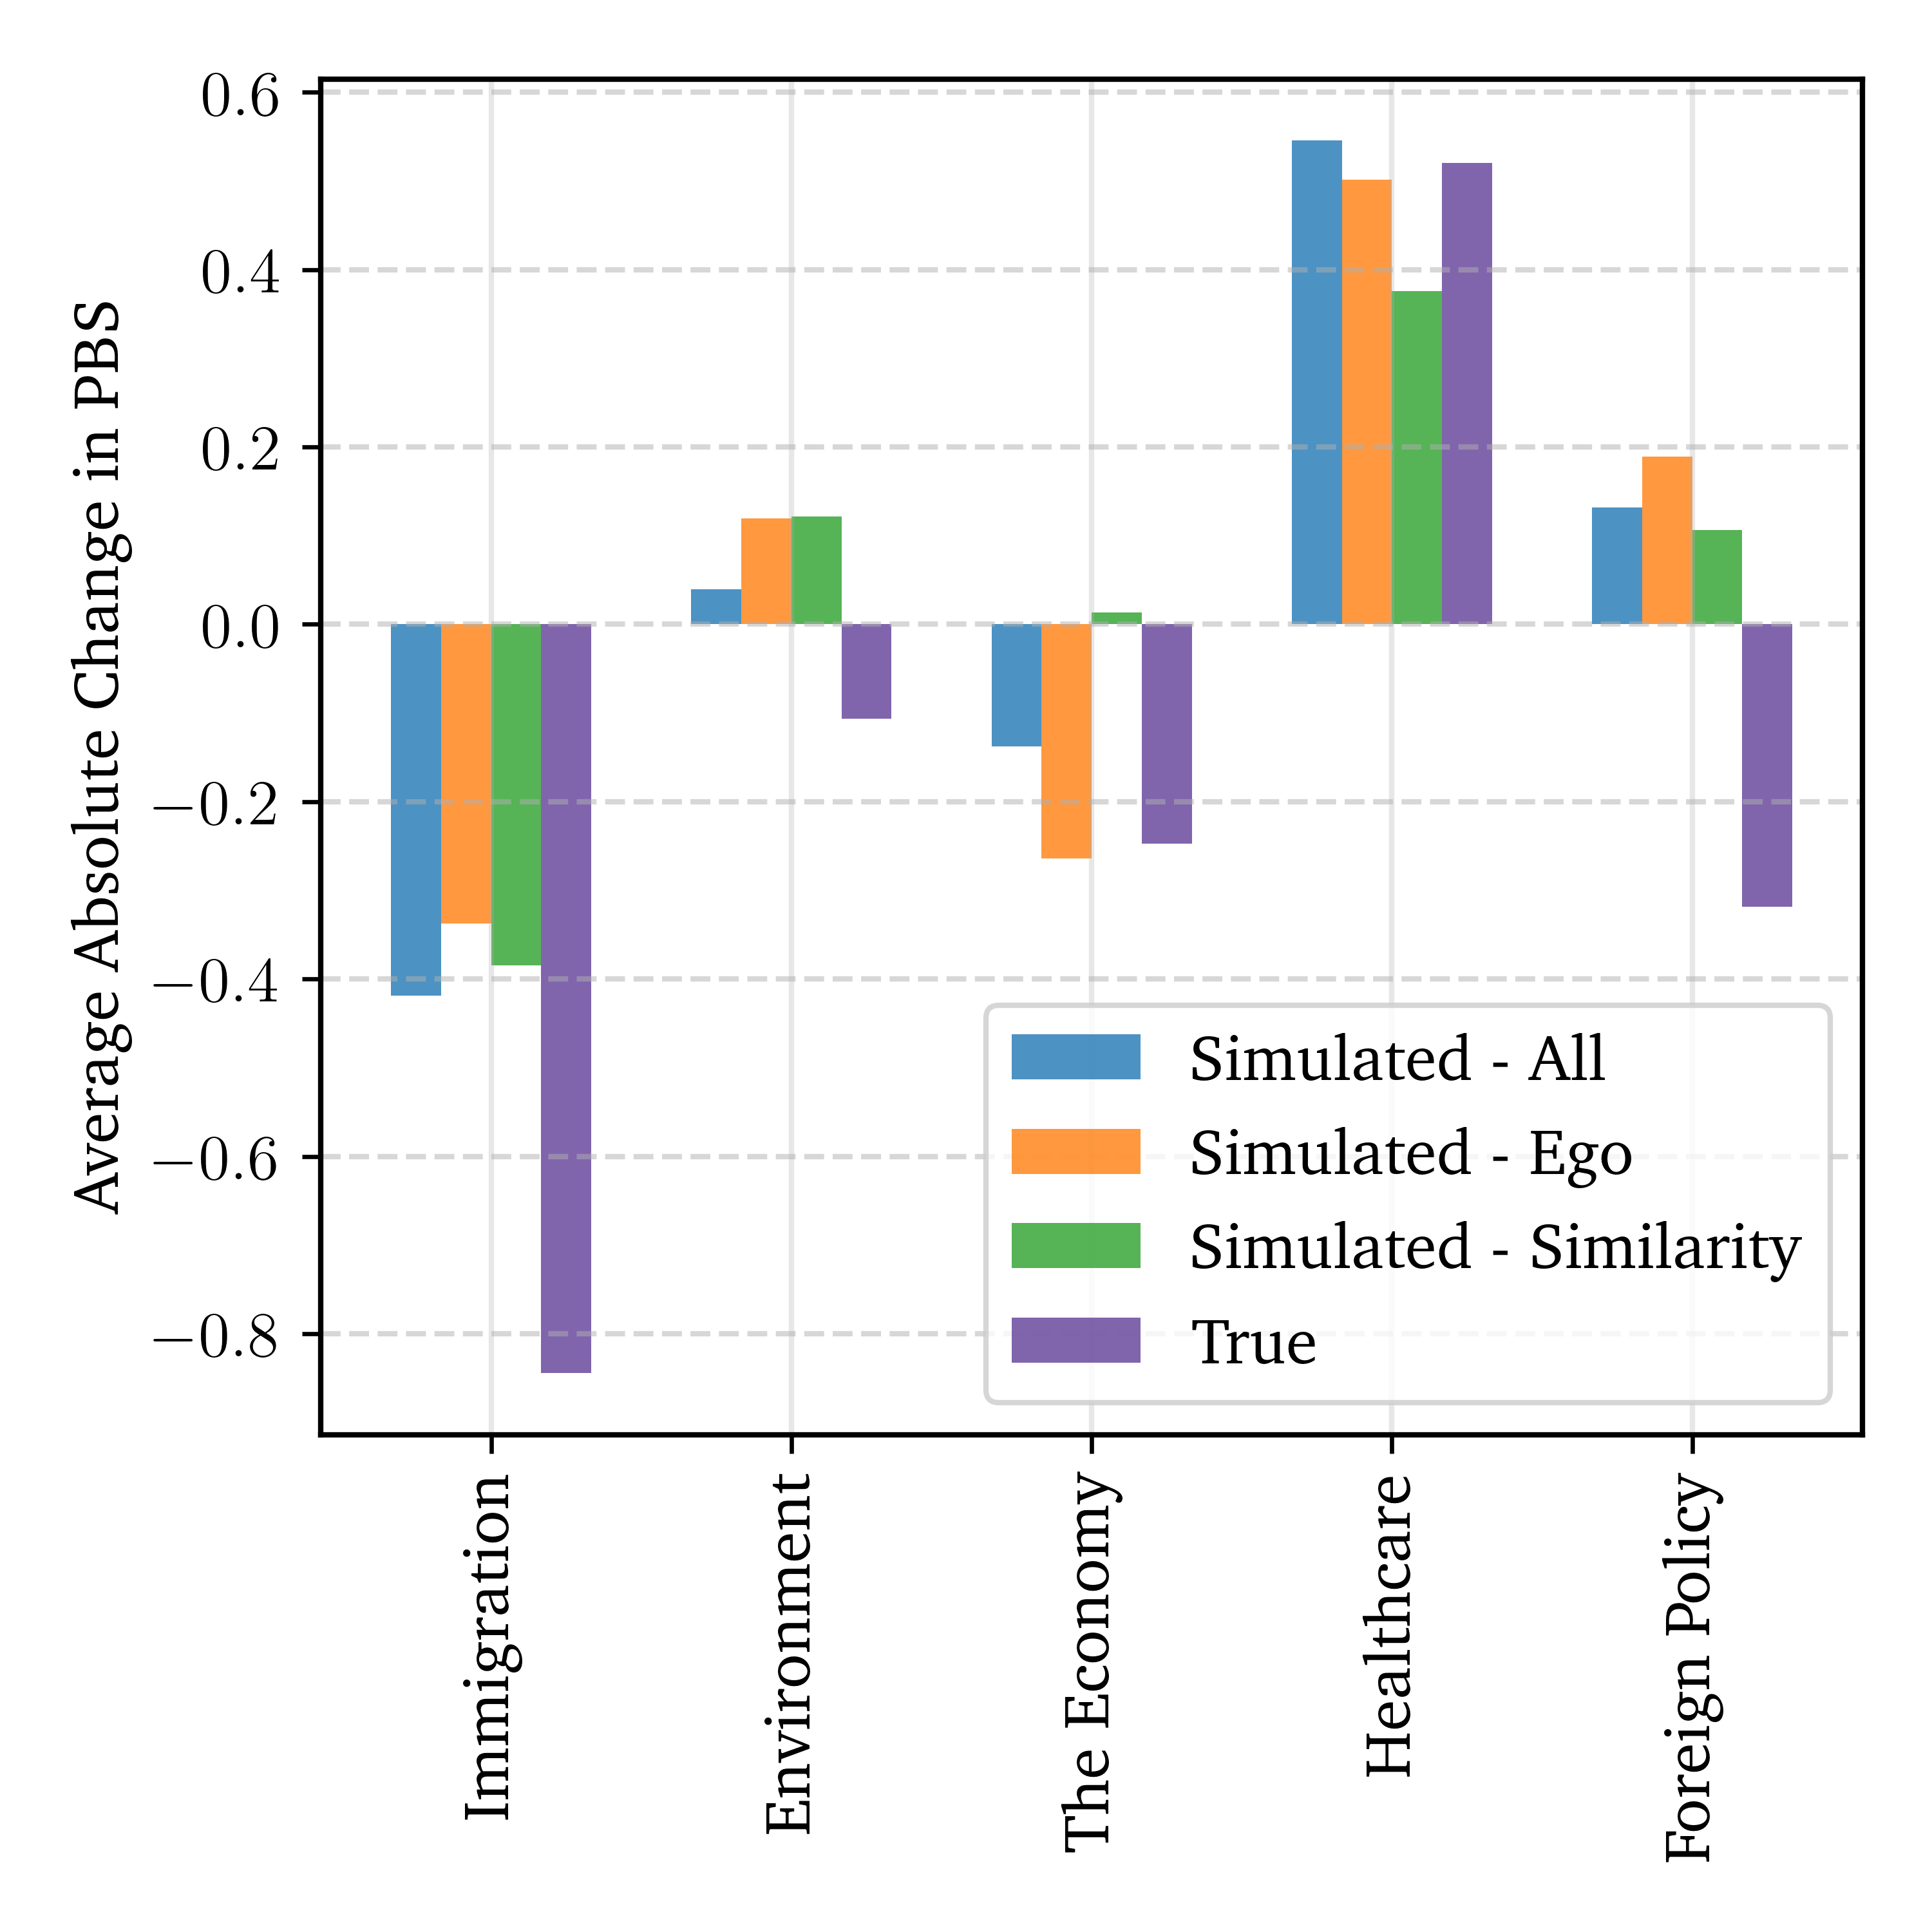
\includegraphics[width=0.6\textwidth]{Figures/per_topic_change.png}
	\end{center}
	\caption{
		Change in PBS per topic with bias random between 0.2 and 0.4. This figure compares the observed change in PBS across policy topics (e.g., healthcare, immigration), showing the average change for three trust mechanisms: ego-based, similarity-based, and the model using all trust signals combined.
	}\label{fig:per_topic}
\end{figure}

\begin{figure}[ht]
	\centering

	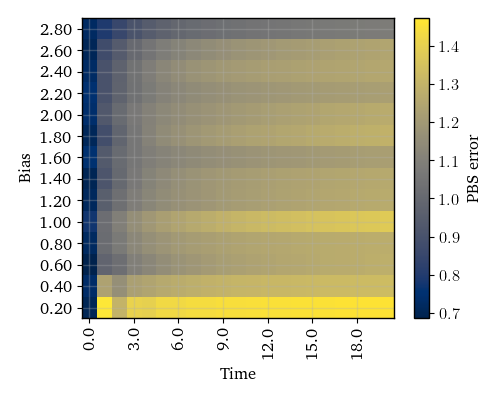
\includegraphics[width=0.6\textwidth]{Figures/bias_time_imshow.png}
	\hspace{1em}
	\caption{Mean absolute prediction error as a function of bias and time using ego based trust. The heatmap shows how the PBS error evolves over time for different bias levels. Higher bias slows the rate of opinion change, and thereby prevents the opinions from becoming homogeneous.}
	\label{fig:bias_slowdown}
\end{figure}

\Cref{fig:bias_slowdown} shows the relation between the bias factor and the
PBS, showing that the bias does not improve the model's predictive power. As
one might expect, bias is ``slowing down'' the model. Because of this, the
model is slower to diverge away from the true opinions.


We suspect ego improves predictive accuracy for two reasons. First, by
assigning individual-specific biases, the model better reflects heterogeneous
deliberative behavior. Second, increased self-bias slows down convergence,
preventing the model from over-correcting.

\subsection{Convergence of Trust Matrices}

From \Cref{theory}, we have seen that in the limit some matrices are
convergent, while some are not, in particular if the matrix is aperiodic, it
is convergent. As we model the deliberation group as having fully connected
matrices, with self-loops, the matrices are aperiodic, and thus convergent. We look at the
distance between the estimated support matrix, and the true support matrix, to
get a sense of the rate of convergence. The distance is defined as the
$\ell_1$ norm.

\begin{figure}[ht]
	\begin{center}
		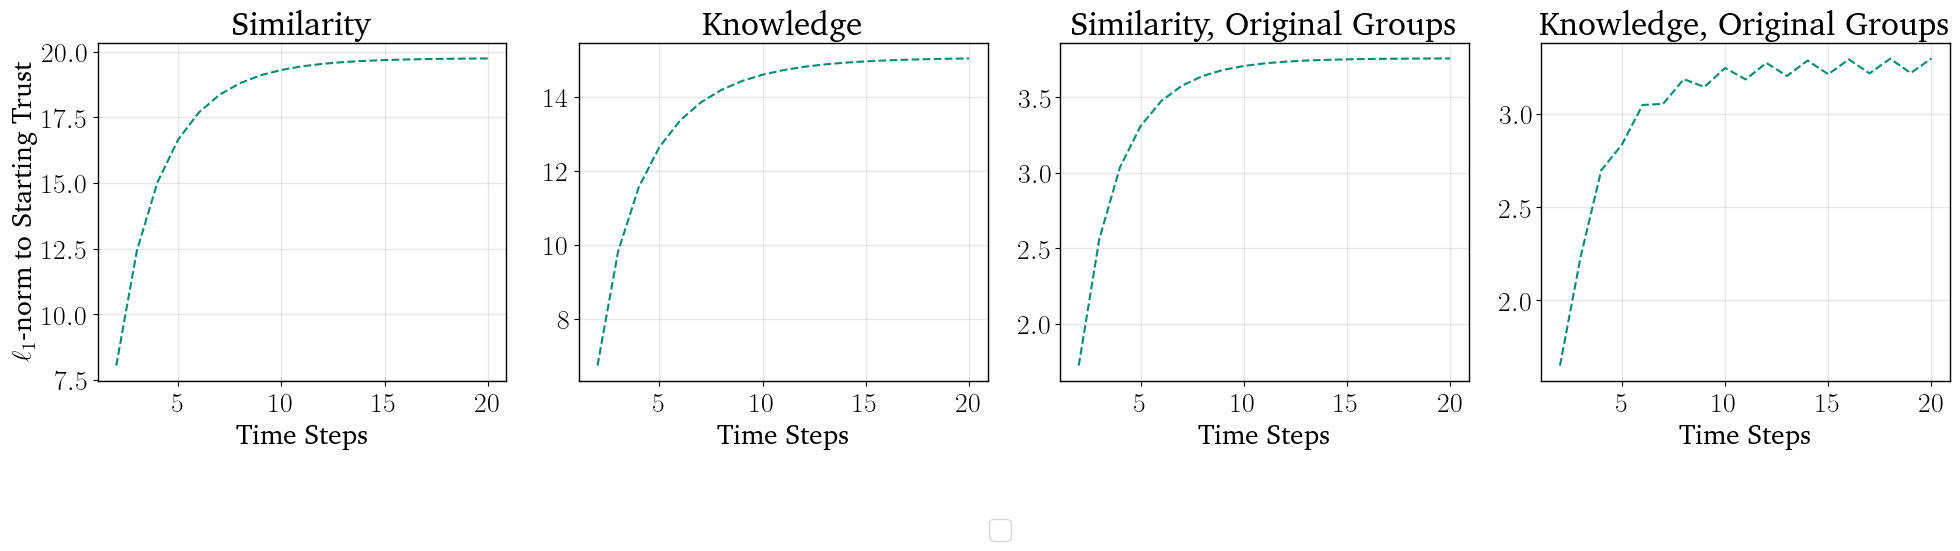
\includegraphics[width=0.95\textwidth]{Figures/convergence_groups.png}
	\end{center}
	\caption{Convergence of trust matrices, as measured by the $\ell_1$-norm between the trust matrix at the start and  trust matrix at the current time step.}\label{fig:convergence_big}
\end{figure}

In \Cref{fig:convergence_big}, all configurations converge at a
similar rate, slowing down the rate of change around t = 15. Since using the
original groups leads to generally smaller groups, the mean absolute difference in
the matrix is smaller. When using knowledge-based trust there is a lower rate
of convergence




\section{Sensitivity Analysis} We perform sensitivity analysis on the predicted
PBS of the model. We do not use the original groups, as this allows us to vary
the number of voters. \Cref{fig:sensitivty_pbs} shows the sensitivity indices.
The first order indices show that the \textit{number
	of voters} is clearly the biggest factor in the variance of the model. As
expected, the \textit{bias} does not directly contribute to the variance in the
model. \textit{Knowledge} informed trust and \textit{self knowledge}
both are significantly impacting the variance of the model.
The second order indices show \textit{number of voters} interacts with
\textit{knowledge}, \textit{self knowledge}, and\textit{ similarity},
contributing a large portion of their explained total variance induced by the
\textit{number of voters}. There is also an interaction between \textit{ego}
and \textit{similarity} and \textit{self knowledge}. As for the Total order
indices, variables contribute significantly to the variance in the
model.

We argue the non-significant first order indices are a result of these
parameters not directly incorporating new information into the model, and thus
on average they do not affect on the outcome. When these parameters are used in
combination parameters that do introduce new information into the model they
start to significantly alter the outcome of the model. As partly supported by
the second order sensitivity indices

\begin{figure}[ht]
	\begin{center}
		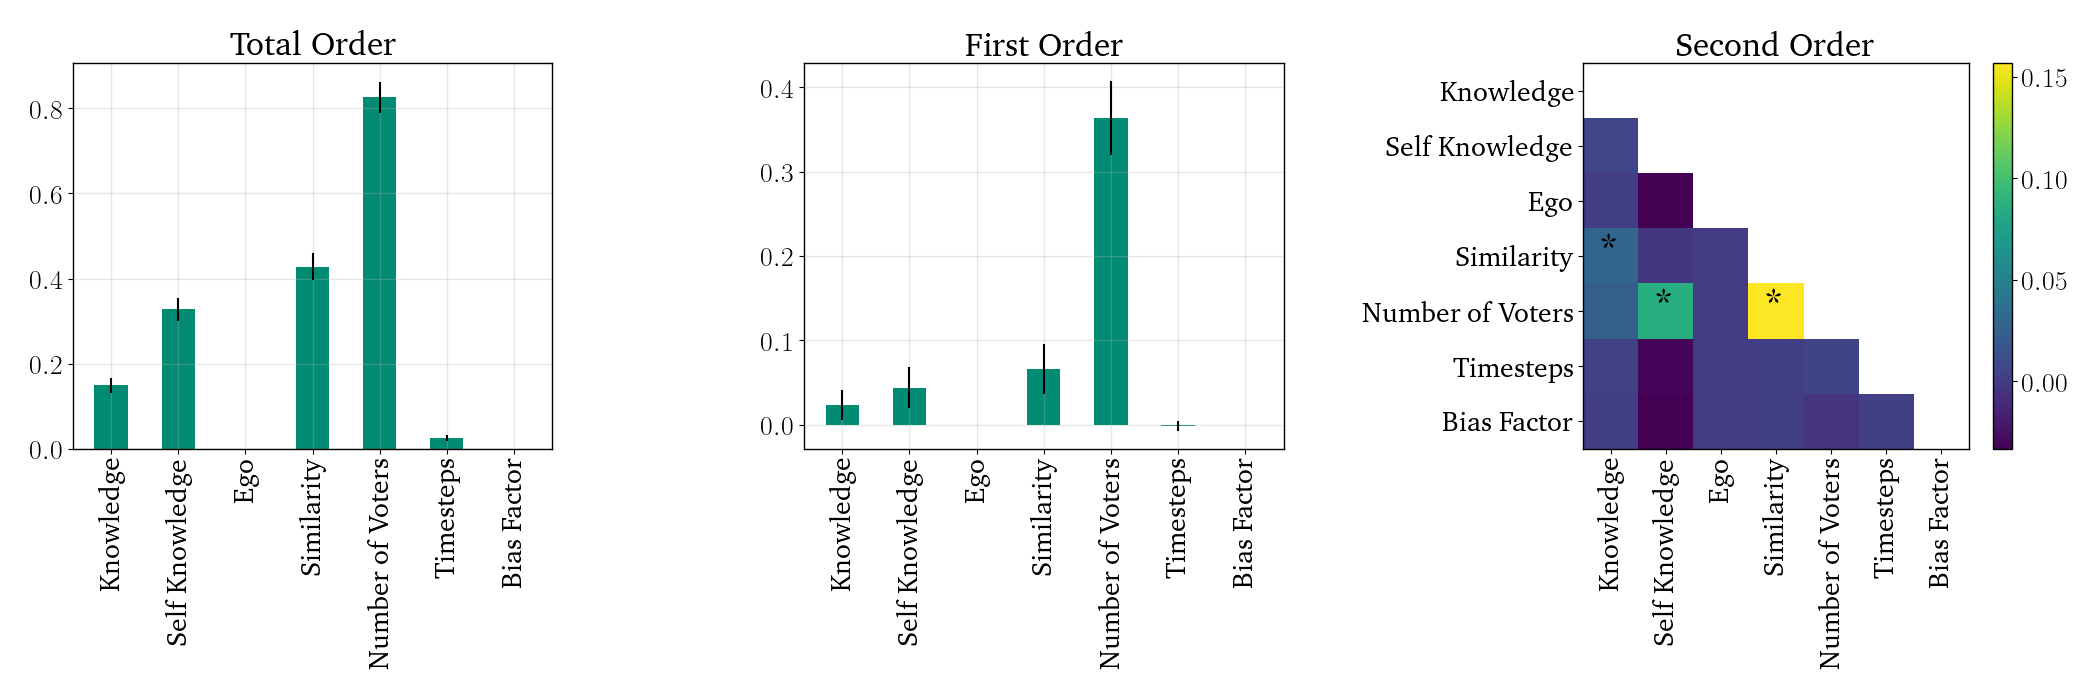
\includegraphics[width=0.95\textwidth]{Figures/senstivity_analysis.png}
	\end{center}
	\caption{Sensitivity indices of parameters influencing PBS prediction error. Asterisks in the second-order panel denote statistically significant interactions. }\label{fig:sensitivty_pbs}
\end{figure}


\section{Adding Meta-Agreement}

\begin{figure}[htbp]
	\centering
	\centering
	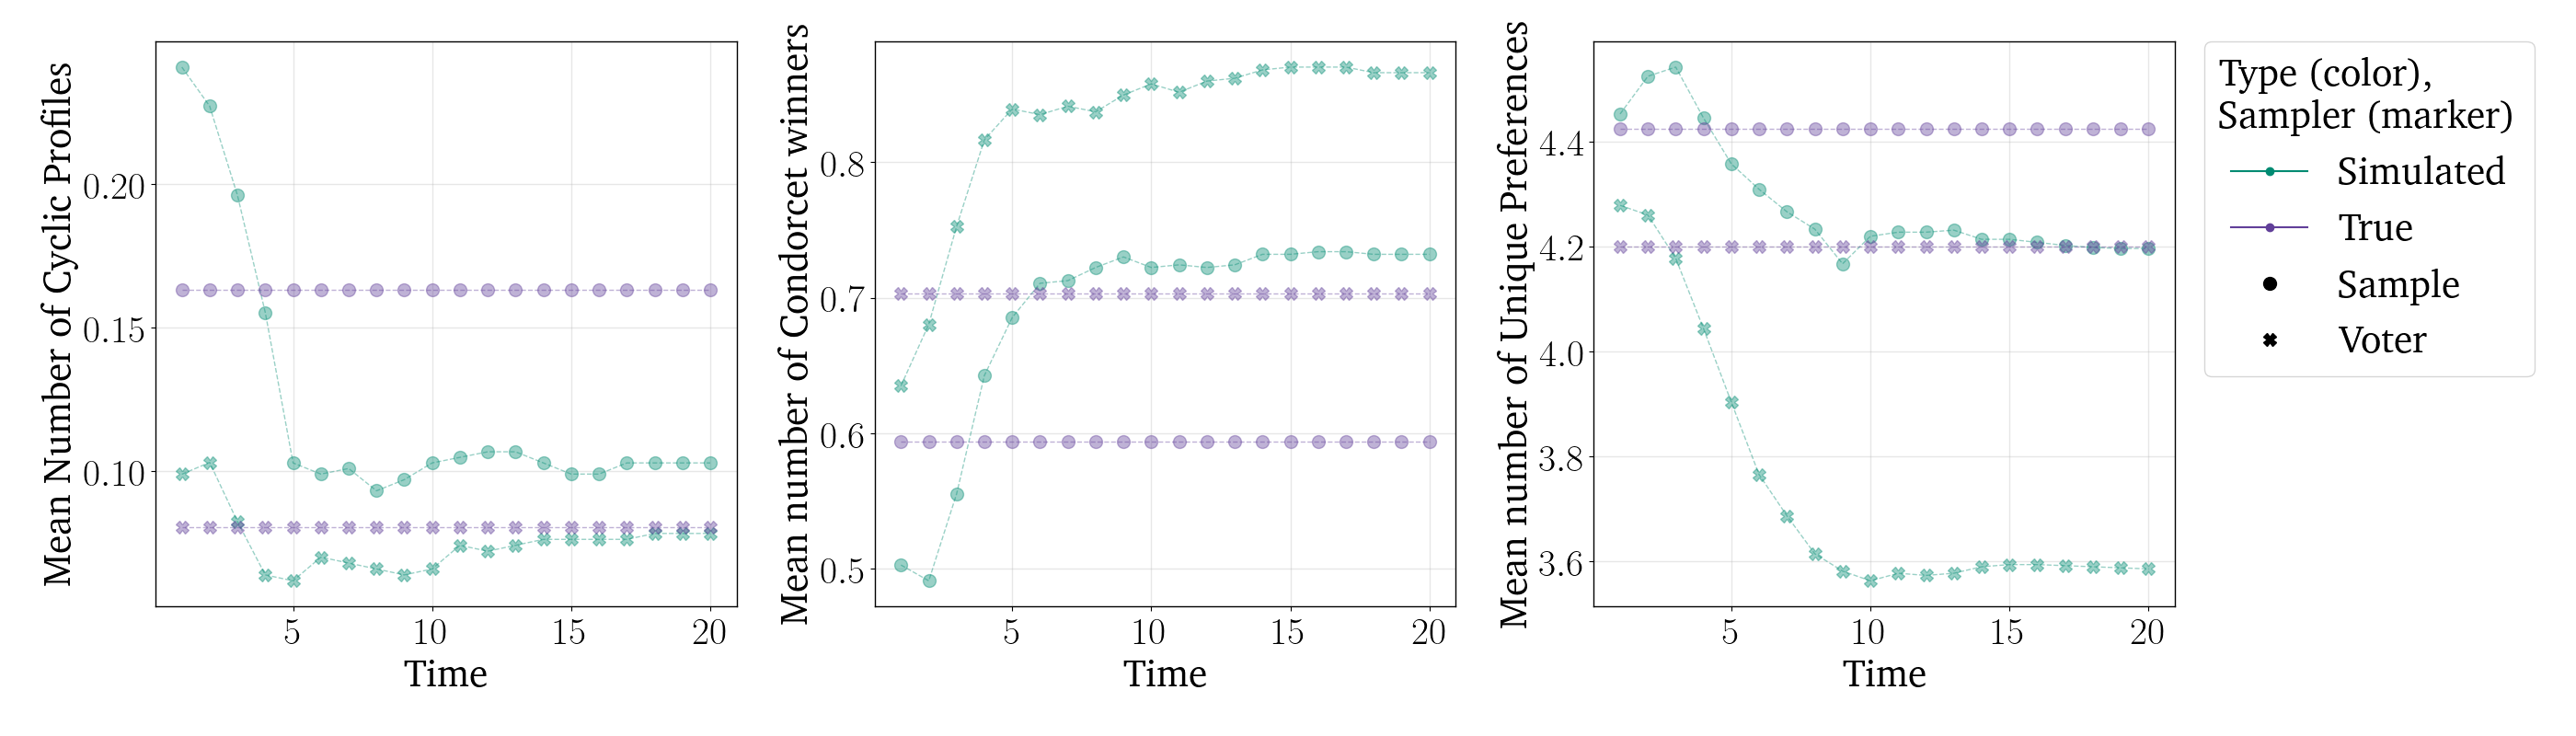
\includegraphics[width=\textwidth]{Figures/three_measures.png
	}
	\caption{Proportion of cyclic profiles in the DeGroot model after adding meta-agreement. Lower values indicate more coherent collective preferences.}
	\label{fig:degroot_cyclic}
\end{figure}

Firstly, when comparing different voter generation mechanisms, we find that generating a candidate by copying the opinion of a single voter performs best—both in minimizing the number of cyclic profiles and in maximizing the frequency with which a Condorcet winner exists. Though this result may seem unintuitive, we suspect the reason is that pre-deliberation opinions were relatively polarized. As a consequence, constructing candidates as averages of 10 voters tends to produce alternatives that are too similar, making it difficult for anyone to stand out.

In contrast, when copying a single voter's opinion, that candidate is more likely to fall near a large
cluster of similar voters, making that candidate closer to the majority. In
such cases, that candidate is more likely to become a Condorcet winner. Put
simply, averaged candidates tend to represent moderate positions, leading to
greater voter indifference between them. In these situations, small errors in
perceived support can have disproportionately large effects. Meanwhile,
candidates based on a single voter's opinion, especially in a polarized
society, are more likely to be distinct and strongly preferred.

Looking at the evaluation metrics used in the model, we observe a pattern
similar to that found in the substantive agreement analysis. The simulation
initially starts far from the true scores, gradually moves toward them,
overshoots, and finally begins to converge.

\begin{figure}[htbp]
	\centering
	\vspace{-9pt}
	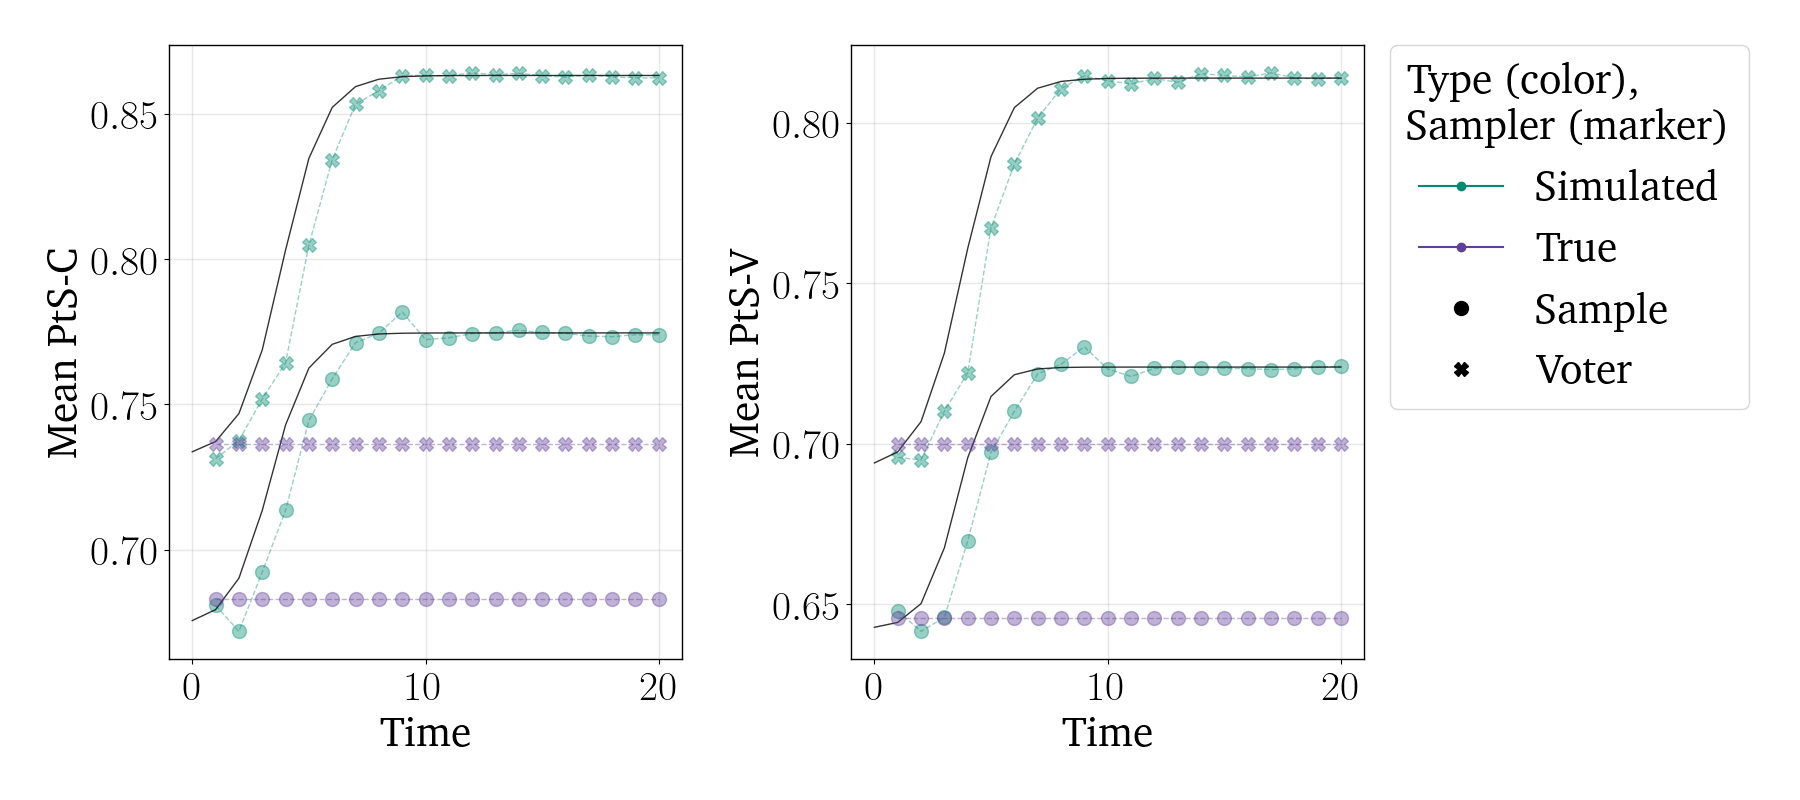
\includegraphics[width=\textwidth]{Figures/pst_measures.png}
	\caption{Proximity to single-peakedness after deliberation via candidate deletion (left) and voter deletion (right). The black line is a fitted sigmoid curve}
	\label{fig:degroot_single_peaked}
\end{figure}

\Cref{fig:degroot_single_peaked} shows similar dynamics across simulation time
for both notions of proximity to single-peakedness. Although candidate deletion
and voter deletion represent two fundamentally different approaches to
measuring this property, they yield a consistent conclusion: voters rapidly
become more single-peaked early in the simulation, after which the rate of
change slows and eventually plateaus. This behavior is well captured by a
sigmoid curve, with an $R^2$ of 0.997 and 0.993 for the PtS-V and PtS-C respectively. The diminishing
rate of change corresponds to the trust matrix stabilizing at its convergent
state.


